\documentclass[10pt,conference]{IEEEtran}

\usepackage{amssymb,amsmath}
\usepackage[T1]{fontenc}
\usepackage{ifpdf}
\usepackage{url}
\ifpdf
\usepackage[pdftex]{graphicx}
\graphicspath{{figs/}}
\DeclareGraphicsExtensions{.png,.jpg, .pdf}
\else
\usepackage[dvips]{graphicx}

\graphicspath{{eps/}}
\DeclareGraphicsExtensions{.eps}
\fi
\usepackage{float}
%\usepackage[caption=false,font=footnotesize]{subfig}
\usepackage[font=footnotesize]{caption}
\usepackage{subcaption}
\usepackage{setspace}
\usepackage{balance}
\pdfminorversion=6
\hyphenation{op-tical net-works semi-conduc-tor}
\newcommand{\indentitem}{\setlength\itemindent{0pt}}
\usepackage{algorithmic}
\usepackage{algorithm}
\newcommand{\algorithmicinput}{\textbf{Input:}}
\newcommand{\INPUT}{\item[\algorithmicinput]}
\newcommand{\algorithmicoutput}{\textbf{Output:}}
\newcommand{\OUTPUT}{\item[\algorithmicoutput]}
\renewcommand{\algorithmicrequire}{\textbf{Pre Condition:}}
\renewcommand{\algorithmicensure}{\textbf{Post Condition:}}
\floatname{algorithm}{Procedure}
\usepackage{tikz}
\usetikzlibrary{matrix,arrows,circuits.ee,circuits.ee.IEC,shapes.geometric,shapes.misc}
\newcommand{\iap}{\textit{DREMS}}
\newcommand{\iapfull}{\textbf{D}istributed \textbf{RE}altime \textbf{M}anaged \textbf{S}ystem}% Algorithmic modifications
\newcommand{\ALOOP}[1]{\ALC@it\algorithmicloop\ #1%
  \begin{ALC@loop}}
\newcommand{\ENDALOOP}{\end{ALC@loop}\ALC@it\algorithmicendloop}
\renewcommand{\algorithmicrequire}{\textbf{Input:}}
\renewcommand{\algorithmicensure}{\textbf{Output:}}
\newcommand{\algorithmicbreak}{\textbf{break}}
\newcommand{\BREAK}{\STATE \algorithmicbreak}
\newenvironment{noindlist}
 {\begin{list}{\labelitemi}{\leftmargin=0.1em \itemindent=0em \itemsep=0.3em}}
 {\end{list}}
\usepackage{multirow}

\begin{document}
\title{Integrated Analysis of Temporal Behavior of Component-based Distributed Real-time Embedded Systems }
\vspace{-0.1in}
\author{\IEEEauthorblockN{Pranav Srinivas Kumar and Gabor Karsai} 
	\IEEEauthorblockA{
		Institute for Software-Integrated Systems\\
		Department of Electrical Engineering and Computer Science\\
		Vanderbilt University, Nashville, TN 37235, USA \\
		Email:\{pkumar, gabor\}@isis.vanderbilt.edu
	}
}

% make the title area
 
\setcounter{page}{1}
\maketitle

\begin{abstract}
%Architecture-oriented domain-specific modeling languages (DSML) can provide a concise and modular abstraction for the structural and behavioral properties of a component-based system. DSMLs are increasingly used in distributed real-time (DRE) systems to manage the complexity and heterogeneity of architectural specifications, both in software and hardware. Such languages also enable model transformations, development automation and design-time analysis before deployment. 

This paper presents a timing analysis approach for modeling and verifying component-based software applications hosted on distributed real-time embedded (DRE) systems. Although schedulability analysis for real-time systems has been a considerably well-studied field, various general-purpose timing analysis tools are not intuitively applicable to all system designs, especially when domain-specific properties such as hierarchical scheduling schemes, time-varying networks and component-based interaction patterns directly influence the temporal behavior. Thus, there is still a need to develop analysis tools that are tightly coupled with the target system paradigm and platform while being generic and extensible enough to be easily modified for a range of systems. In this context, we have developed a Colored Petri Net-based schedulability analysis tool that integrates with a domain-specific modeling language and component model and that simulates and verifies temporal behavior for component operations in mission-critical DRE systems. Our results show the scalable utility of this approach for preemptive and non-preemptive hierarchical scheduling schemes in distributed scenarios.
\end{abstract}

\begin{IEEEkeywords}
	component-based, real-time, distributed, colored petri nets, 
	timing, schedulability, analysis
\end{IEEEkeywords}
\section{Introduction}

Real-time systems, by definition, must meet operational deadlines. These deadlines constrain the amount of time permitted to elapse between a stimulus provided to the system and a response generated by the system. Delayed responses or missed task deadlines can have catastrophic effects on the function of the system, especially in the case of safety- and mission-critical applications. This is the primary motivation for design-time schedulability analysis and verification of systems. 

There is a wealth of existing literature studying real-time task scheduling theory and timing analysis in uniprocessor and multiprocessor systems \cite{Audsley1995, Sha2004}. There are also several modeling, schedulability analysis and simulation tools \cite{MAST1, Cheddar, TIMES, PTIDES} that address various challenges in verifying real-time requirements although many such tools are appropriate only for certain task models, interaction patterns, scheduling schemes, or analysis goals. For component-based architectures, model-based system designs are usually expressed in a formal domain such as timed automata \cite{Alur1994, Macariu2010}, controller automata \cite{Zhang2012}, high-level Petri nets \cite{masri2009} etc. so that existing analysis tools such as UPPAAL \cite{UPPAAL} or CPN Tools \cite{CPNTools} can be used to verify either the entire system or its compositional parts. But, it is also evident that many of the existing schedulability analysis tools, though grounded in theory are not directly applicable to all system designs, especially with respect to domain-specific properties such as component interaction patterns, distributed deployment, time-varying communication networks etc. 

To be useful, the analysis tools need to be tightly integrated with the target domain: the concurrency model used by the system. The classic thread-based concurrency model (with generic synchronization primitives) is too low-level and too generic, it is hard to use, and hard to analyze. For pragmatic reasons, more restrictive, yet useful concurrency models are needed for which dedicated analysis tools can be developed. Our previous efforts \cite{MoDeVVa} were directed at this challenge. The target domain for that study was the DREMS component model \cite{DREMS13Software} which is the foundation of a software infrastructure addressing challenges in the design, development, and deployment of component-based embedded software for distributed applications like flight software for fractionated spacecraft. The physical nature of such systems requires strict, accurate and pessimistic timing analysis at design-time to avoid catastrophic situations at run-time. DREMS is implemented as a design-time tool suite and a run-time software platform that is enhanced by a component (concurrency) model with well-defined execution and interaction semantics. The platform relies on a temporally partitioned task scheduling scheme, a non-preemptive component-level operations scheduler, support for various communication and interaction patterns; all deployed on a distributed hardware platform.

Our contributions in this paper target efficient modeling and analysis techniques of temporal behavior for component-based applications that form distributed real-time embedded systems, such as DREMS. 

\begin{enumerate}
	\item We present an approach for modeling  the 'business logic': the operational behavior of each component in an application. The model uses a sequence of timed steps that are executed in the course of a component operation, including steps that specify interactions with other components. This approach enables abstracting the details of the middleware, while representing the temporal behavior of the component business logic. 
	\item We also present improvements to the CPN-based modeling approach that enables better analysis performance and scalability. These rely on heuristics that manage time variables and state space data structures more efficiently. 
	\item We also present advanced state space analysis methods and tools applied on the modeled system to reduce analysis time on medium to large-scale systems.
\end{enumerate}

The rest of this paper is organized as follows. Section \ref{sec:Related_Research} presents related research, reviewing and comparing existing analysis tools and formal methods. Sections \ref{sec:Target_System_Architecture} briefly describes the DREMS architecture, specifically the concepts of interest that are covered by the timing analysis tool. Section \ref{sec:Modeling} describes the business logic modeling approach to capture the operational behavior of components in the application. Section \ref{sec:Analysis} describes the analysis improvements we were able to achieve with structural changes to the analysis model. This section also briefly describes the application of advanced state space analysis methods that enable efficient state space searches while reducing the state space size and overall memory consumption. Section \ref{sec:Future_Work} evaluates possible extensions to this work before concluding with Section \ref{sec:Conclusions}.
\section{Related Research}
\label{sec:Related_Research}

% MAST
Verification of component-based systems requires significant amount of information about the application assembly, interaction semantics, and real-time properties. This information is primarily derived from the design model although many real-time metrics are not explicitly modeled. Using model descriptors, \cite{Lopez2006} describes interaction semantics and real-time properties of components. Using the MAST modeling and analysis framework \cite{MAST1, MAST2}, schedulability analysis and priority assignment automation is supported. Event-driven models are separated into several \emph{views} which are similar to hierarchical pages in some modeling formalisms, like Colored Petri Nets (CPN). Analysis efforts include the calculation of response times, blocking times, and slack times. %For every real-time application, a separate and independent real-time analysis model is generated for each mode of operation and analyzed

High-level Petri nets are a powerful modeling formalism for concurrent systems and have been integrated into many modeling tool suites for design-time verification. General-purpose Architecture Analysis \& Design Language (AADL) models have been translated into symmetric nets for qualitative analysis \cite{kordon_sn} and Timed Petri nets \cite{kordon2009} to check real-time properties such as deadline misses, buffer overflows etc. Similar to \cite{kordon2009}, our CPN-based analysis also uses bounded observer places \cite{Alpern1989} that observe the system behavior for property violations and prompt completion of operations. However, \cite{kordon2009} only considers periodic threads in systems that are not preemptive. Our analysis is aimed at a combination of preemptive and non-preemptive hierarchical scheduling with higher-level component interaction concepts. separately.

Several analysis approaches present tool-aided methodologies that exploit the capabilities of existing analysis and verification techniques. In the verification of timing requirements for composed systems, \cite{medina2011} uses the OMG UML Profile for Modeling and Analysis of Real-Time and Embedded Systems (MARTE) modeling standard and converts high-level design into MAST output models for concrete schedulability analysis. In a similar effort, AADL models are translated into real-time process algebra \cite{sokolsky2006} reducing schedulability analysis into a deadlock detection problem searching through state spaces and providing failure scenarios as counterexamples. Symbolic schedulability analysis has been performed by translating the task sets into a network timed automata, describing task arrival patterns and various scheduling policies. TIMES \cite{TIMES} calculates worst-case response times and scheduling policies by verifying timed automata with UPPAAL \cite{UPPAAL} model checking.

In order to analyze hierarchical component-based systems, the real-time resource requirements of higher-level components need to be abstracted into a form that enables scalable schedulability analysis. The authors in \cite{easwaran2006} present an algorithm where component interfaces abstract the minimum resource requirements of the underlying components, in the form of periodic resource models. Using a single composed interface for the entire system, the component at the higher level selects a value for operational period that minimizes the resource demands of the system. Such refinement is geared towards minimum waste of system resources.

\section{Target System Architecture}
\label{sec:Target_System_Architecture}
The target architecture for timing analysis is \emph{DREMS} \cite{ISIS_F6_Aerospace:12,DREMS13Software}. DREMS is a software infrastructure for the design, implementation, deployment, and management of component-based real-time embedded systems. The infrastructure includes (1) design-time modeling tools \cite{ISIS_F6_SFFMT:13} that integrate with a well-defined (2) component model \cite{ISIS_F6_ISORC:13, MoDeVVa} used to build component-based applications. Rapid prototyping and code generation features coupled with a modular run-time platform automate tedious aspects of software development and enable robust deployment and operation of mixed-criticality distributed applications. The formal modeling and analysis method presented in this paper focuses on applications built using this foundational architecture. We emphasize here the importance of a component model: it defines a model of computation with a strict component execution semantics. 

\subsection{Component Operations Scheduler}

DREMS applications are built by assembling and composing re-useable units of functionality called \emph{Components}. Each component is characterized by a (1) set of communication ports, a (2) set of interfaces (accessed through ports), a (3) message queue, (4) timers and state variables. Components interact via publish/subscribe and synchronous or asynchronous remote method invocation (RMI and AMI) patterns. Each component interface exposes one or more \emph{operations} that can be invoked. Every operation request coming from an external entity reaches the component through its message queue. This is a priority-based queue maintained by a component-level scheduler that schedules operations for execution. When ready, a single \emph{component executor thread} per component will be released to execute the operation requested by the front of the component's message queue. The operation runs to completion, hence component execution is always single-threaded. Note however that the multiple components \emph{can} be executed concurrently. 


\subsection{Operating System Scheduler}
DREMS components are grouped into processes that are assigned to ARINC-653 \cite{ARINC-653} styled temporal partitions, implemented by the DREMS OS scheduler. Temporal partitions are periodic, fixed intervals of the CPU's time. Threads associated with a partition are scheduled only when the partition is active. This enforces a temporal isolation between threads assigned to different partitions and assigns a guaranteed slice of the CPU's time to that partition. The repeating partition windows are called \emph{minor frames}. The aggregate of minor frames is called a \emph{major frame}. The duration of each major frame is called the \emph{hyperperiod}, which is typically the lowest common multiple of the partition periods. Each minor frame is characterized by a period and a duration. The duration of a partition defines the amount of time available per hyperperiod to schedule all threads assigned to that partition. Each \emph{node} in a network runs an OS scheduler, and the temporal partitions of the nodes are assumed to be synchronized, i.e. all hyperperiods start at the same time. 

\subsection{Colored Petri Nets}

Petri nets \cite{Murata1989} are a graphical modeling tool used for describing and analyzing a wide range of systems. A Petri net is a five-tuple $(P, T, A, W, M_0)$ where $P$ is a finite set of places, $T$ is a finite set of transitions, $A$ is a finite set of arcs between places and transitions, $W$ is a function assigning weights to arcs, and $M_0$ is the initial marking of the net. Places hold a discrete number of markings called tokens. Tokens often represent resources in the modeled system. A transition can legally fire when all of its input places have necessary number of tokens. 
% Simplify...
%Since Petri net tokens are not distinguishable, the obtained model is often too complex for large systems. To enable compact representations for the modeled system, extensions to the basic Petri net model, called high-level Petri nets, are preferred.
With Colored Petri nets (CPN) \cite{CPN}, tokens contain values of specific data types called \emph{colors}. Transitions in CPN are enabled for firing only when valid colored tokens are present in all of the typed input places, and valid arc bindings are realized to produce the necessary colored tokens on output places. The firing of transitions in CPN can check for and modify the data values of these colored tokens. Furthermore, large and complex models can be constructed by composing smaller sub-models as CPN allows for hierarchical description. %This extended paradigm can more easily model and analyze systems with typed parameters. 


\section{Analysis Challenges}
\label{sec:Challenges}

There are certain implicit design complexities in DREMS that motivate our modeling and analysis approach.
\subsection{Operation Deadlines}
\label{subsec:Operation_Deadlines}
For each component the executor thread, when released by the component-level scheduler, runs under the control of the (fine-grain) OS scheduler. Each component executor thread has a fixed priority, assigned at design-time. However, the deadline for it is determined by the operation it executes, maintained at a higher level of abstraction. Therefore, depending on the operation executed by the executor thread, its timing requirements vary.

\subsection{WCET of Operations}
The execution of component operations serve the various periodic or aperiodic interaction requests from either the underlying framework or other connected (possibly distributed) components. Each operation is written by an application developer as a sequence of execution \emph{steps}. Each step could execute a unique set of tasks, e.g. perform a local calculation or a library call, initiate an interaction with another component, process a response from external entities, and it can have data-dependent, possibly looping control flow, etc. The behavior derived by the combination of these steps dictates the WCET of the component operation. This behavior includes non-deterministic delays that are caused by components communicating through a (1) time-varying network (2) using specific interaction patterns and (3) within the constraints of temporally partitioned execution. 

%System architectures like DREMS require an analysis tool with an expressive language that is tightly coupled with the target software platform (like our component model) to efficiently model and verify behavioral aspects of the system such as operational modes, the OS scheduling and distributed communication. Another crucial need for safety-critical systems is incorporating the timing analysis in every stage of the design. This firstly requires an analysis tool that can work with the non-determinism realized by incomplete designs. Secondly, this also requires the timing specifications and model transformations to be integrated into the design-time modeling. All of these aspects motivated us to choose colored Petri nets as the formalism to capture the various domain-specific properties and perform efficient timing analysis.


\section{Colored Petri Net-based Analysis Model}
\label{sec:Colored_Petri Net-based_Analysis_Model}

This section briefly describes how Colored Petri nets (CPN) are used to build an extensible, scalable analysis model for component-based applications. Several nets are used to compose the different layers of the design model. To edit, simulate and analyze this model, we use the CPN Tools \cite{CPNTools} tool suite. The tool suite includes a simulator, as well as a state-space analysis tool that computes the (bounded) state space of the system under execution. The analysis model is based on the formal component model, i.e. the model of computation used. For a different component execution semantics, this model needs to be adjusted. 

\subsection{Model of Time}
Appropriate choice for temporal resolution is a necessary first step in order to model and analyze threads running on a processor. The OS scheduler enforces temporal partitioning and uses a priority-based scheme for threads active within a temporal partition. If multiple threads have the same priority, a round-robin (RR) scheduling is used. In order to observe and analyze this behavior, we have chosen the temporal resolution to be 1 ms; a fraction of 1 clock tick of the OS scheduling quantum. 
\subsubsection{Dynamic Time Progression}
Although the time resolution at the start of the analysis is chosen to be 1 ms, this is not a constant throughout the execution of the analysis model. If it were then \emph{S} seconds of activity will generate a state space of size: $SS_{size} = \sum\limits_{i=1}^{S*1000} TF_{t_i}$
%\vspace{-0.2in}
%
%\begin{equation}
%\begin{split}
%SS_{size} = \sum\limits_{i=1}^{S*1000} & TF_{t_i}
%\end{split}
%\end{equation}
where $TF_{t_i}$ is the number of state-changing CPN transition firings between $t_i$ and $t_{i+1}$. This large state space includes intervals of time where there is no thread activity to analyze either due to lack of operation requests, lack of ready threads for scheduling, or due to temporal partitioning. During such idle periods, the analysis engine dynamically increases the time-step size and progresses time either to (1) the next node-specific clock tick, (2) the next global timer expiry offset, or (3) the next node-specific temporal partition (whichever is earliest and most relevant). This ensures that the generated state space tree is devoid of nodes where there is no thread activity. Such dynamic control of time using global variables during analysis is also one of the advantages of using colored Petri nets. 

\subsection{Modeling Component-based Applications}

\begin{figure}[htb]
	\centering
	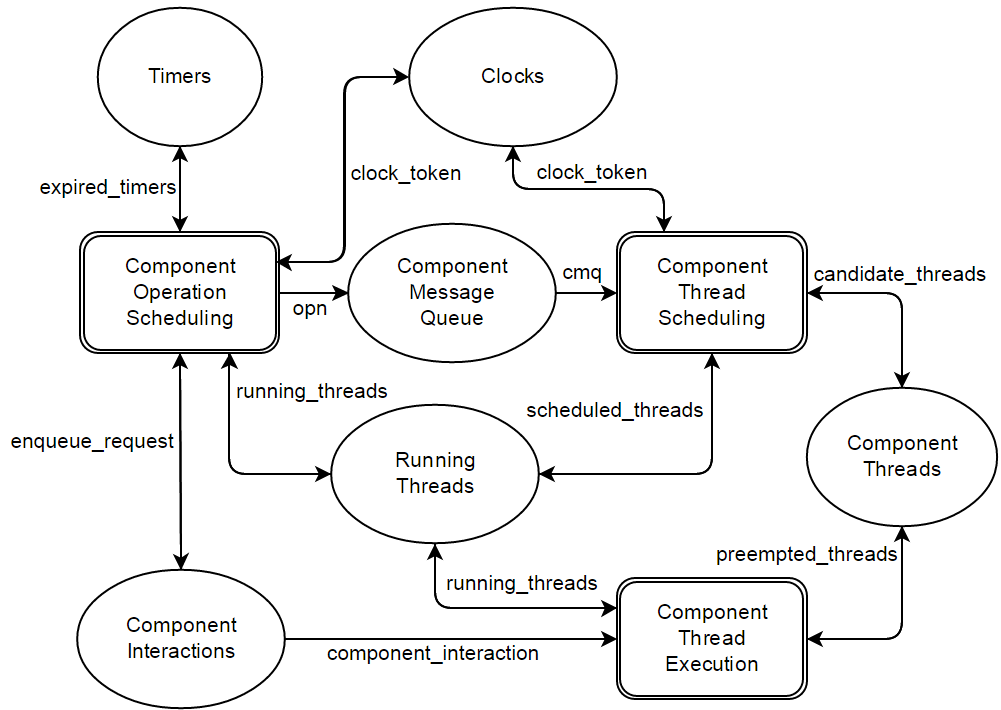
\includegraphics[width=0.45\textwidth]{figs/HL_CPN.png}
	\caption{Top-level CPN Model}
	\label{fig:hl_cpn}
\end{figure}

The top-level CPN Model is shown in Figure \ref{fig:hl_cpn}. The places (shown as ovals) in this model maintain \emph{colored} (typed) tokens that represent the states of interest for analysis. For instance, the \emph{Clocks} place holds tokens of type \emph{clock\_tokens} maintaining information regarding the state of the clock values and temporal partition schedule on all computing nodes. To ensure modularity, this model is partitioned into two interacting sub-nets to handle the hierarchical scheduling.

\subsubsection{Component-level Execution Model}

\paragraph{Component Operations} Every operation request \emph{O} made on a component \emph{$C_x$} is a \emph{record} type implementation of the 4-tuple:

\vspace{-0.15in}
\begin{equation}
O(C_x) = \ < ID_O, \ Prio_O, \ Dl_O, \  Steps_O >
\end{equation}

where, $ID_O$ is a unique concatenation of strings that help identify and locate this operation in the system (consisting of the name of the operation, the component, the computing node, and the temporal partition). The operation's priority ($Prio_O$) is used by the analysis engine to enqueue this operation request on the message queue of $C_x$ using a fixed-priority non-preemptive FIFO scheduling scheme. The completion of this enqueue implies that this operation has essentially been \emph{scheduled} for execution. Once enqueued, if this operation does not execute and complete before its fixed deadline ($Dl_O$), its real-time requirements are violated. 

\paragraph{Steps} 
\label{para:steps}

Once an operation request is dequeued, the execution of the operation is modeled as a transition system that runs through a sequence of steps dictating its behavior. Any of these underlying steps can have a state-changing effect on the thread executing this operation. For example, interactions with I/O devices on the component-level could block the executing thread (for a non-deterministic amount of time) on the OS-level. Therefore, every component operation has a unique list of steps ($Steps_O$) that represent the sequence of local or remote interactions undertaken by the operation. Each of the \emph{m} steps in $Steps_O$ is a 4-tuple:

\vspace{-0.15in}
\begin{equation}
s_i = \ <Port, \ Unblk_{s_i}, \ Dur_t, \ Exec_t>
\end{equation}

where $1 \le i \le m$. \emph{Port} is a \emph{record} representing the exact communication port used by the operation during $s_i$. $Unblk_{s_i}$ is a list of component threads that are unblocked when $s_i$ completes. This list is used, e.g., when the completion of a synchronous remote method invocation on the server side is expected to unblock the client thread that made the invocation. Finally, temporal behavior of $s_i$ is captured using the last two integer fields: \emph{$Dur_t$} is the worst-case estimate of the time taken for $s_i$ to complete and $Exec_t$ is the relative time of the execution of $s_i$, with $0 \le Exec_t \le Dur_t$.

\paragraph{Component Interactions}

Consider an application with two components: a client and a server. The client is periodically triggered by a timer to make an remote method call to the server. We know that when the client executes an instance of the timer-triggered operation, a related operation request is enqueued on the server's message queue. In reality, this is handled by the underlying middleware. Since we do not model the details of this framework, the server-side request is modeled as an \emph{induced operation} that manifests as a consequence of the client-side activity. Tokens that represent such design-specific interactions are maintained in the place \emph{Component Interactions} (Figure \ref{fig:hl_cpn}) and modeled as shown in equation \ref{eq:component_interactions}. The interaction \emph{Int} observed when a component $C_x$ queries another component $C_y$ is modeled as the 3-tuple:

\vspace{-0.15in}
\begin{equation}
\label{eq:component_interactions}
Int(C_x, C_y) = \ < Node_{C_x}, \ Port_{C_x}, \ O(C_y)>
\end{equation}

When an operational \emph{step} in component $C_x$ uses port $Port_{C_x}$ to invoke an operation on component $C_y$, the request $O_{C_y}$ is enqueued on the message queue of $C_y$. %As shown in Figure \ref{fig:hl_cpn}, the transition \emph{Component Operation Scheduling} observes the \emph{Running Threads} at every time step to check for completion of external interaction requests. When satisfied, the necessary operation token is removed from \emph{Component Interactions} and enqueued onto the appropriate message queue.

\paragraph{Timers}

DREMS components are inactive initially; once deployed, a component executor thread is not eligible to run until there is a related operation request in the component's message queue. To start a sequence of component interactions, periodic or sporadic timers can be used to trigger a component operation. In CPN, each timer $TMR$ is held in the place \emph{Timers} and represented as shown in Eq. \ref{eq:TMR}. Timers are characterized by a period ($Prd_{TMR}$) and an offset ($Off_{TMR}$). Every timers triggers a component using the operation request $O_{TMR}$.

\vspace{-0.15in}
\begin{equation}
\label{eq:TMR}
TMR = \ < Prd_{TMR}, \ Off_{TMR}, \ O_{TMR}>
\end{equation}

\subsubsection{OS-level Execution Model}

\paragraph{Temporal Partitioning}
The place \emph{Clocks} in Figure \ref{fig:hl_cpn} holds the state of the node-specific global clocks. The temporal partition schedule modeled by these clocks enforces a constraint: component operations can be scheduled and component threads can be run only when their parent partition is active. Each clock token \emph{NC} is modeled as a 3-tuple:

\vspace{-0.15in}
\begin{equation}
\label{eq:NC}
NC = \ < Node_{NC}, \ Value_{NC}, \ TPS_{Node_{NC}} >
\end{equation}

where, $Node_{NC}$ is the name of the computing node, $Value_{NC}$ is an integer representing the value of the global clock and $TPS_{Node_{NC}}$ is the temporal partition schedule on $Node_{NC}$. Each \emph{TPS} is an ordered list of temporal partitions.

\vspace{-0.15in}
\begin{equation}
\label{eq:TP}
TP = \ < Name_{TP}, \ Prd_{TP}, \ Dur_{TP}, \ Off_{TP}, \ Exec_{TP} >
\end{equation}

Each partition $TP$ (Eq. \ref{eq:TP}) is modeled as a record color-set consisting of a name $Name_{TP}$, a period $Prd_{TP}$, a duration $Dur_{TP}$, an offset $Off_{TP}$ and the state variable  $Exec_{TP}$. %Aggregate of such partitions can fully describe a partition schedule. Complete partition schedules are maintained per computing node.

\paragraph{Component Thread Behavior}

Figure \ref{fig:Thread_Execution} presents a simplified version of the CPN to model the thread execution cycle. The place \emph{Component Threads} holds tokens that keep track of all the ready threads in each computing node. Each component thread $CT$ is a record characterized by:

\vspace{-0.15in}
\begin{equation}
\label{eq:CT}
CT = \ <ID_{CT}, \ Prio_{CT}, \ O_{CT}>
\end{equation}

where $ID_{CT}$ constitutes the concatenation of strings required to identify a component thread in CPN (i.e. component name, node name and partition). Every thread is characterized by a priority ($Prio_{CT}$) which is used by the OS scheduler to schedule the thread. 
%The DREMS OS uses a fixed-priority preemptive scheduling scheme (constrained by temporal partitioning) to schedule component threads. %If multiple threads belonging to the same temporal partition are ready, the highest priority thread is always chosen for execution. If there is more than one candidate thread, one is chosen at random, followed thereafter by a Round-Robin scheduling scheme. 

\vspace{-0.1in}
\begin{figure}[htb]
	\centering
	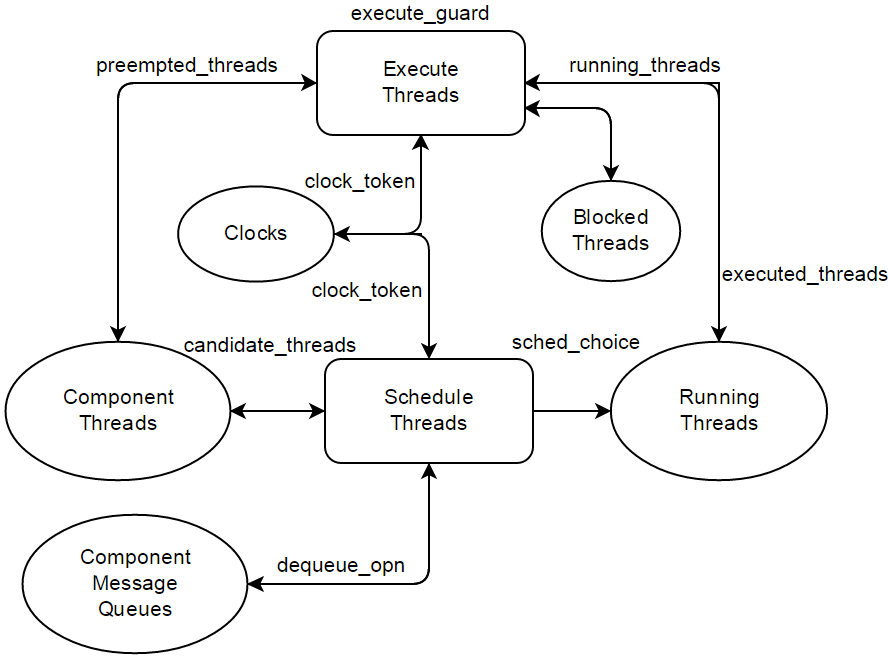
\includegraphics[width=0.40\textwidth]{figs/Thread_Execution.png}
	\caption{Component Thread Execution Cycle}
	\label{fig:Thread_Execution}
\end{figure}

If the highest priority thread is not already servicing an operation request, the highest priority operation from \emph{Component Message Queues} is dequeued and scheduled for execution (held by $O_{CT}$). The scheduled thread is placed in \emph{Running Threads}. %The guard on \emph{Schedule Thread} ensures that the highest priority thread in the currently running partition is scheduled first. 

When a thread token is marked as running, the model checks to see if the thread execution has any effect on itself or on other threads. These state changes are updated using the transition \emph{Execute Thread} which also handles time progression. Keeping track of $Value_{NC}$, the thread is preempted at each clock tick. This loop repeats forever, as long as there are no system-wide deadlocks. 

%It must be noted that system-critical processes such as deployment and fault management processes running periodically (or sporadically) at higher priorities than component processes are not necessarily affected by temporal partitioning. Such processes are scheduled to execute in a \emph{SYSTEM} partition when ever ready. Therefore when simulating the scheduling of such process threads, $TPS_{Node_{NC}}$ in equation \ref{eq:NC} is ignored.





\chapter{State Space Analysis and Verification}
\label{chapter:analysis}

The state of a dynamic system refers to a minimal set of variables, called state variables, that fully describe the system and its response to any given set of inputs. This minimum set of variables, $s_i(t), i=0,1,2,..n$ along with knowledge of those variables at an initial time $t_0$ and the system inputs for time $t > t_0$, are sufficient to predict the future system state and outputs for all time $t > t_0$. This asserts that the dynamic behavior of a state is completely characterized by the set of state variables $s_i(t)$. 

CPN Tools uses a built-in \emph{state space} analysis tool to generate a bounded state space from an initialized CPN model. Here, the state space is a directed graph structure where the vertices, called states, each represent a unique system state. An edge between two states represents the transition from one state to another. If a state $S$ can non-deterministically transition into $K$ possible future states, then $S$ becomes the root of a K-ary tree. The state of the system in our case is a record of all the places in the CPN i.e. the token values in every place of the CPN model. This record is therefore a snapshot of the token configuration of the net and represents its execution state. State space generation is a process of generating this directed graph, from some initial state. State spaces of dynamic systems can be potentially infinite if there is always a potential unique state transition. For pragmatic reasons, we generate a bounded state space i.e. a graph structure bounded by some rule e.g. $t_i < t_bound$, where $t_i$ is some global time variable. In this case, the state space will contain only nodes where the state variable $t_i$ is less than some upper bound $t_bound$. Alternately, the rule can be to generate a state space as long as the component message queue size is under 50 waiting requests. 

To illustrate the state space analysis of DREMS using our CPN, we consider a simple example -- consider three equal-priority components, grouped into a process and executed on a single device. Each component has a periodic timer that fires every 10 ms and triggers the respective components into executing a block of code. Each component maps to an executor thread and these three threads are scheduled concurrently with all other threads in the system. In this example, there are no other component threads or system-level threads considered. Based on the OS scheduling scheme, these components, with equal priority, are scheduled using round-robin conflict resolution i.e. one of these threads is chosen at random and then a cyclic scheduling order is maintained. Since all three timers have the same period, the three timers fire concurrently and the respective component threads are marked as 'ready' at the exact same time. Since all three component threads are ready to execute the same times, there are $3!$ possible thread execution orders in the worst case when following round-robin scheduling. 

Figure \ref{fig:SSScreenshot} shows a bounded state space generated in CPN Tools for this component assembly. There are 6 branches from the initial state of the system as the model realizes the 6 possible behaviors. Each node in this state space is annotated with a state space ID and also a pair of integers in the format \emph{"p:c"}, where p refers to the number of parent nodes and c refers to the number of child nodes. This figure also shows results of a \emph{state space query}. Specifically, the query finds the \emph{marking} on the \emph{Completed\_Operations} place in two different state space nodes, 35 and 37. In node 37, Timer\_3\_operation is the first operation to complete as Component\_3 is the first ready thread chosen by the OS. In node 35, Timer\_1\_operation is the first operation to complete as Component\_1 is the first ready thread chosen by the OS. This illustrates the tree of possible behaviors that is encoded in the state space starting from an initial state. The goal of state space analysis is to search this tree of possibilities to identify a single execution trace i.e. a single branch in this tree that either satisfies or negates a system property e.g. that the deadline of one of these timer operations is violated. 


\begin{figure}[htb]
	\centering
	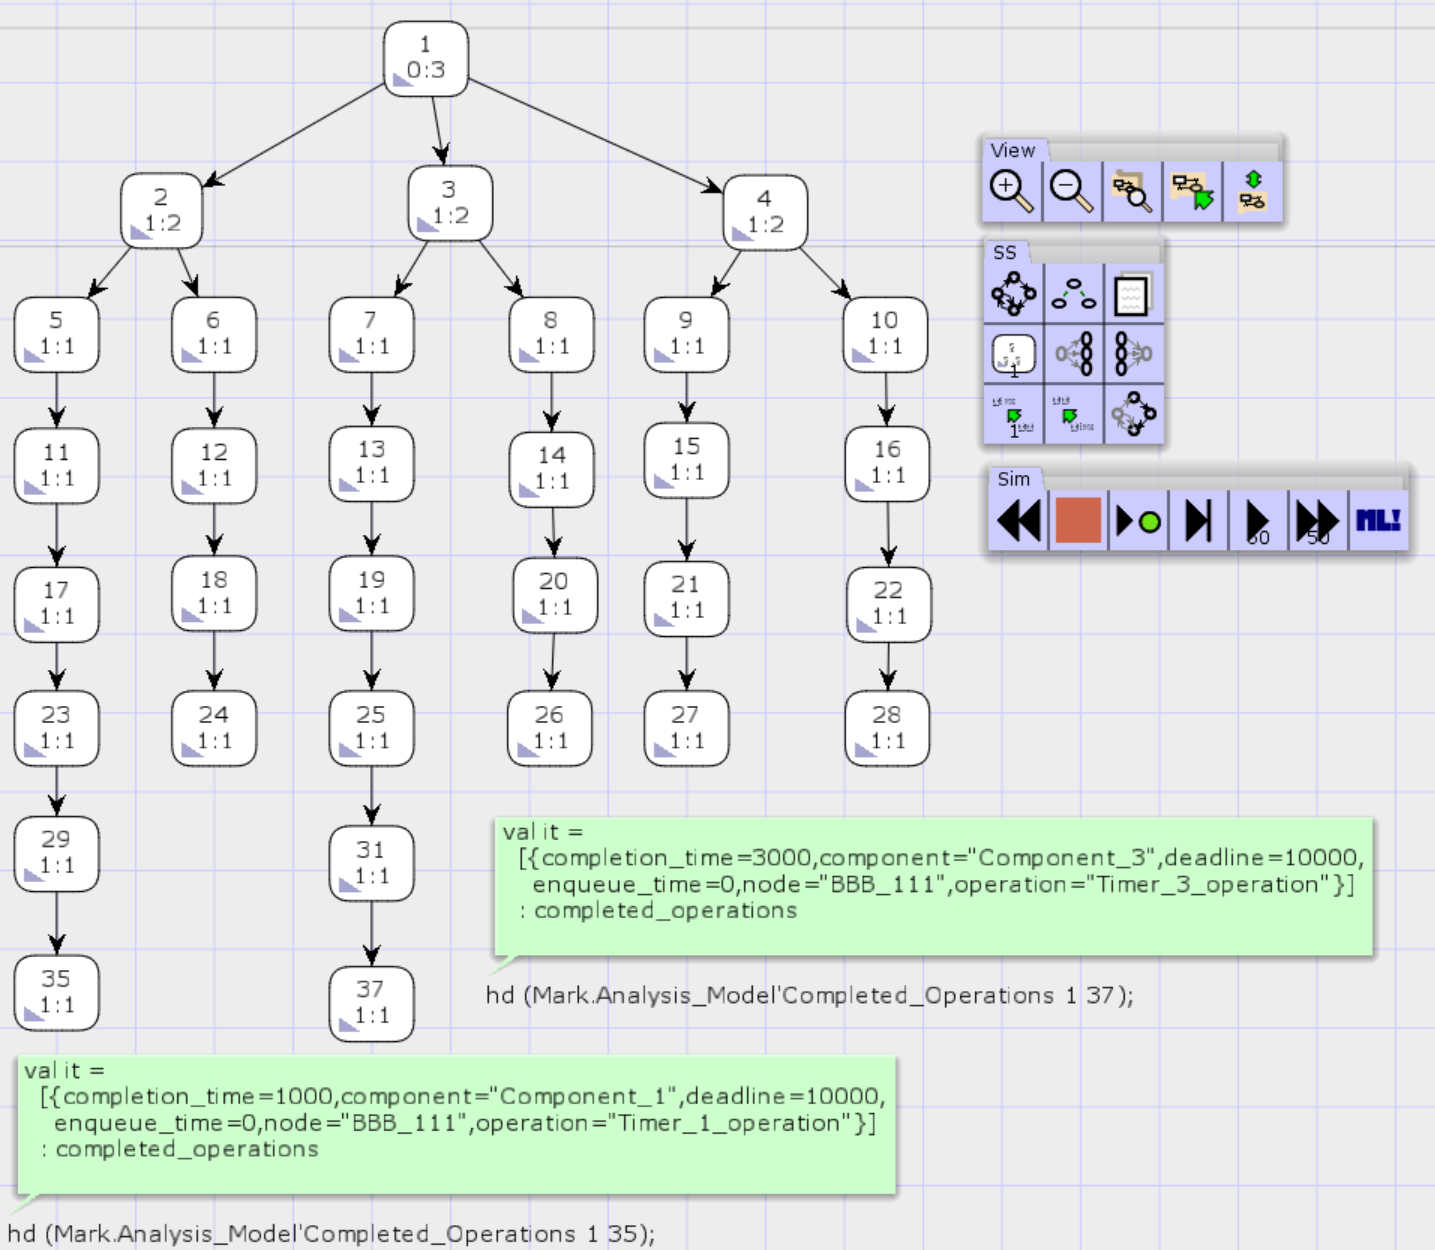
\includegraphics[width=\textwidth]{./img/state-space-analysis.png}
	\caption{Bounded State Space for a Multi-component Timer example -- The component threads have the same real-time priority and are executed in the same device. Each component is triggered with a 100 Hz periodic timer and all three timers are synchronized to illustrate non-determinism. The round robin  scheduling quantum is set to 4 milliseconds. 'Mark' is a state space query function that provides the \emph{marking} of a place in a particular state space node.}
	\label{fig:SSScreenshot}
\end{figure}
\FloatBarrier

\subsection{Searching the State Space}

CPNTools' inbuilt state space analysis tool comes with a programming interface -- a set of function that can be used by a user to query a generated state space. One of the many available functions is the \emph{SearchNodes} function, as shown in Figure \ref{fig:SSSearching}. This function traverses the nodes of the state space and at each node, evaluates a predicate and accumulates a list of nodes that satisfy this predicate. 

\begin{figure}[htb]
	\centering
	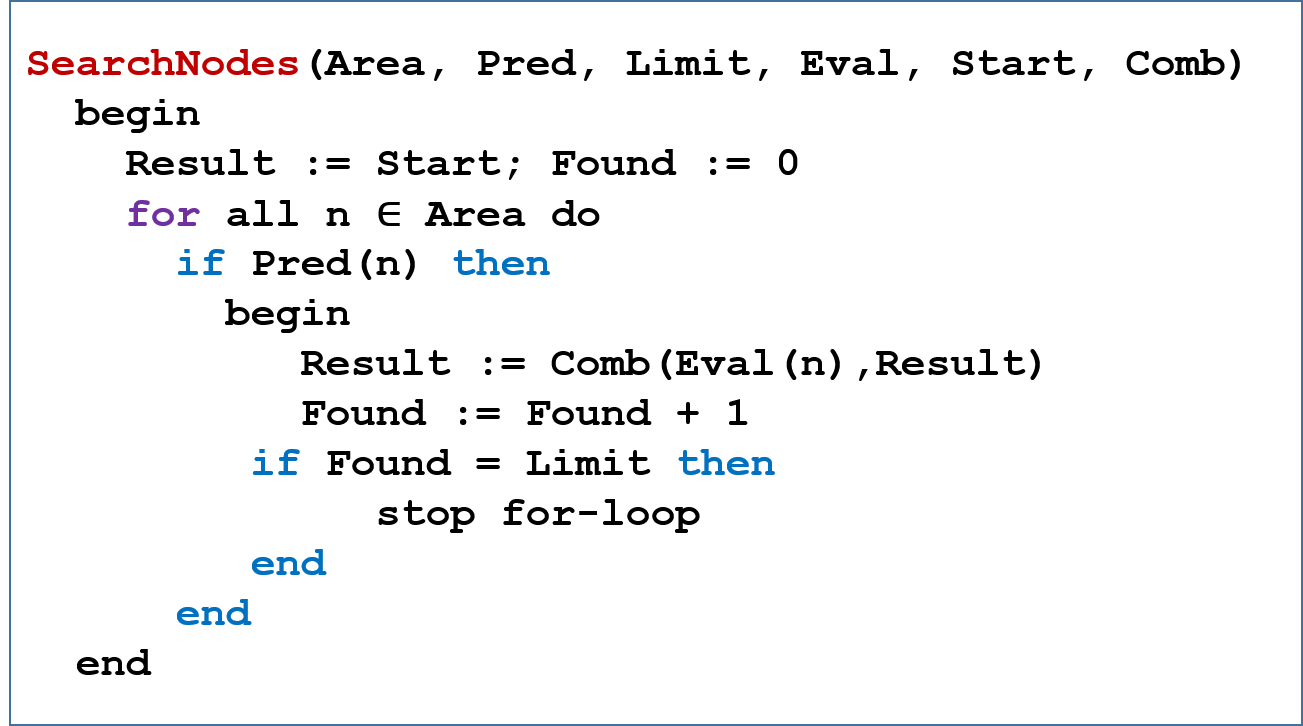
\includegraphics[width=0.7\textwidth]{./img/state-space-searching.png}
	\caption{SearchNodes function provided by CPNTools}
	\label{fig:SSSearching}
\end{figure}
\FloatBarrier

There are six parameters provided to this search function. \emph{Area} refers to the search area i.e. the part of the state space that needs to be searched. Often, the search area is the entire graph but it is possible to provide a subset of the graph e.g. a list of strongly connected components \footnote{A directed graph $G$ is strongly connected if every vertex is reachable from every other vertex in the graph. A strongly connected component is a maximal strongly connected subgraph of $G$ i.e. no additional edges or vertices from $G$ can be included in the subgraph without breaking its property of being strongly connected}. The second argument, emph{Pred}, specifies a predicate function that evaluates each node and produces a boolean result. All nodes that evaluate to false are ignored and all nodes that evaluate to true are retained for further analysis. The third argument, \emph{Limit} is an integer referring to how many times a predicate should evaluate to true before the search should terminate. If this limit is infinite, the entire state space is always searched. \emph{Eval} is an evaluation function that is executed on all state space nodes that satisfy the predicate function e.g. an evaluation function to find the execution time of an operation when its predicate function detects a deadline violation. Lastly, \emph{Start} is the initial value of the result and \emph{Comb} is a combination function that accumulates each new result from the evaluation function with prior results. The combination function is a constant time operation as it simply appends a new node to the end of the accumulated results list. The search algorithm itself has a time complexity of $O(n)$ where $n$ is the number of nodes in the state space. 

The rest of this chapter details how a bounded state space can be used to analyze DREMS applications for deadline violations, response times predictions etc. 

\subsection{Deadline Violations}

A \emph{deadline violation} refers to a system state where the execution time of a component operation has exceeded its deadline. The operation may violate its deadline without beginning execution since wait times in the message queue count towards the total delay from the arrival of the message to the completion of the corresponding operation. The SearchNodes function in CPNTools is quite generic and can be easily applied to our analysis model to identify such violations in the state space. For all operations, either completed or waiting for execution, it is sufficient to execute the predicate $current\_time - operation.enqueue_time > operation.deadline$. All nodes that satisfy this predicate are nodes that represent deadline violation states. 

Alternatively, by adding observer places to our timing analysis model i.e. places that passively observe the system and accumulate tokens when certain conditional transitions execute, deadline violations can be recorded as the model is executing. A \emph{Deadline\_Violation} (Figure \ref{fig:DL}) transition fires at any point in time when the guard \emph{dl\_guard} is satisfied and arc bindings are realized with its input places. The transition observes the states of the currently running threads and the component message queues to identify deadline violations on operations that are either executing or waiting to execute. The \emph{dl\_violation} tokens in \emph{Late Operations} ($LO$) is of the form:

\begin{equation}
\label{eq:DLV}
LO = \ <Node_{name}, O_{name}, O_{ST}, \ O_{DLT}>
\end{equation}

where operation $O_{name}$ executing on computing node $Node_{name}$ started at time $O_{ST}$ and violated its deadline at time $O_{DLT}$. Since the component-level scheduler uses a non-preemptive scheme, this operation is still run to completion after the violated deadline. Delays like these propagate to the waiting operations in the message queue.

\begin{figure}[htb]
	\centering
	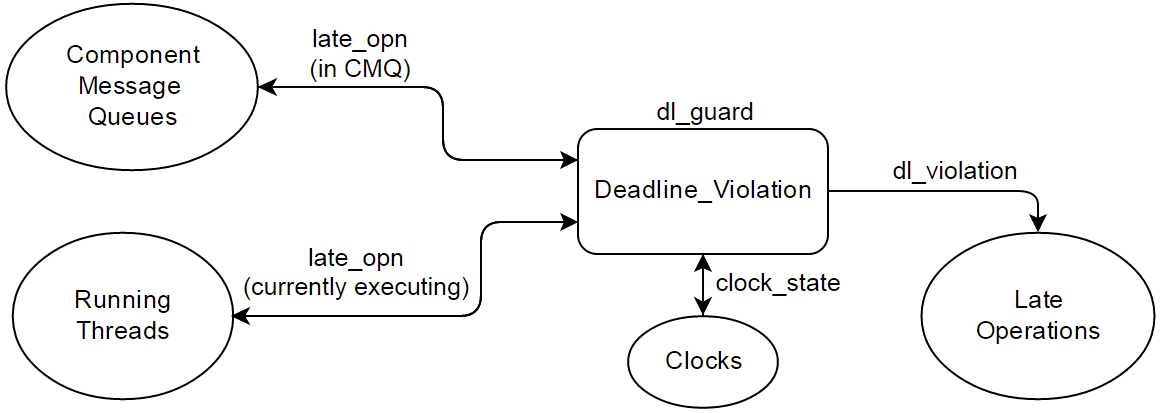
\includegraphics[width=\textwidth]{./img/Deadline_Violations.png}
	\caption{Deadline Violation Observer place}
	\label{fig:DL}
\end{figure}
\FloatBarrier

\subsection{System-wide Deadlocks}

System-wide deadlocks are caused by the inability of the OS schedulers (on all nodes) to schedule any component thread. This can be caused by situations where a set of executing threads are indefinitely blocked on each other because of cyclic dependencies in the interactions. Deadlocks can be identified by checking the leaf nodes of the bounded state space for \emph{dead transitions} that are unable to fire. Alternatively, the tokens in \emph{Component Interactions} are analyzed to identify cyclic dependencies and provide warnings to possible deadlocks. Such queries are useful in large component assemblies where mutually blocking dependencies are not immediately perceivable. 

\subsection{Response-time Analysis}

Response time analysis identifies the worst-case time taken for the system to generate a desired output signal after an input trigger has been provided e.g. time taken for the emergency braking system on an automated train controller to respond to sensory input. A component-based system can have a variety of triggers but in this context, a trigger is considered as any operation request received by a component. The response to this trigger is the completion of some other operation at a future time instant after the occurrence of the trigger. With state space analysis, it is possible to identify the worst-case response times for a $(trigger\_operation, response\_operation)$ pair by first obtaining response times for all trigger-to-response cycles and finding the maximum. 

Similar to deadline violation detection, using the SearchNodes function, this can be accomplished as follows -- The predicate function for the search is the completion of the response\_operation. The evaluation function scans the list of completed operations in all state space nodes where a response operation was the last operation marked as completed. In this list, by identifying the trigger operation and response operation, the response time is calculated as the difference $Response\_Operation_{cmpl\_time} - Trigger\_Operation_{enq\_time}$. This result is accumulated by the combination function and the maximum response time is calculated from the resultant list. The time complexity of this search is again linear with respect to the size of the state space. The size of the accumulated results list is at most half the size of the state space since the trigger and the response are always in separate state space nodes. Finding the maximum trigger-to-response time within the resultant list is also done in linear time.   

This result, as with other state space analysis results here, assumes ideal functional behavior for all operations i.e. the completion of the operation always provides the desired results. Since the business logic model for operations does not encode data-dependent behavior and conditional execution, the completion of a response operation is no indication about the correctness of the response, merely its timeliness. It is therefore also not possible to differentiate between response "types" as all responses are seen as equivalent. 

\subsection{Incomplete Designs}

As shown in Figure \ref{fig:SSScreenshot}, the state space generated by the timing analysis model contains all possible branches of execution from an initial system state. By encoding system requirements as predicates, it is possible to obtain useful analysis results that can aid system integrators in better designing components. When designing component-based systems, it is often the case where priorities need to be assigned to component threads executing on the same device, especially in real-time systems. These priorities are typically estimated based on relative importance of operations, order of component interactions, and frequency of associated triggers. An ideal priority assignment is one that leads to the most efficient schedule, one that avoids resource starvation while ensuring that the assignment does not violate any timing requirements. In large-sized component assembly, it is not always clear what each component's priorities should be. State space analysis can be useful here in providing a partial thread execution ordering based on the timing requirements of component operations. 

In Figure \ref{fig:SSScreenshot}, if the deadline i.e. timing requirement, of Timer\_1\_operation was 1 ms, then the thread ordering analysis would always suggest executing Component\_1 first before other components - essentially suggesting a higher priority for Component\_1 if this timing requirement is paramount. Furthermore, timing requirements can be ranked based on importance. A global timing requirement spanning distributed applications may be more important than a local timing requirement that is within the scope of a single component. To achieve this, the state space analysis identifies state space nodes where an operational timing requirement is satisfied and presents the order of thread execution on that device. By comparing such orderings with other ordering where such timing requirements fail, a system integrator obtains a partial execution order for threads. Using this result as feedback, the integrator can change the relevant component priorities and repeat the analysis. 


\section{Modeling and Analysis Improvements}
\label{sec:Improvements}

\subsection{Problem Statement}

The CPN analysis work presented in \cite{kumar2014colored} has some limitations. The clock values in the distributed set of computing nodes progress by a fixed amount of time regardless of the pace of execution. This is one of the primary causes of state space explosion since many of the intermediate states between \emph{interesting} events, though uneventful, are still recorded by the state space generation. For instance, in a temporal partition spanning 100 ms, even if a thread executes for 5 ms and the rest of the partition is empty, then if the clock progresses at a 1 ms rate, a 100 states are recorded in the state space when there are at most 5-7 interesting events in this interval. For a larger set of distributed interacting components, this can become a problem. Also, for distributed scenarios where multiple instance of a set of applications are executed in parallel, in independent computers, our CPN modeling methodology isn't efficient, leading to a tree of parallel executions even when the distributed computers are independent i.e. the computers can be synchronously progressed. The goal of this work is to mitigate such analysis issues and arrive at a more efficient and scalable analysis model. 

\subsection{Outline of Solution}
Improving the performance of our CPN analysis method required the evaluation of our existing results to identify how the state space generation worked. The state space of CPN is a tree of CPN \emph{markings}, where each marking is a data structure representing the tokens in all it's places. So, our goal is to reduce the number of markings accumulated in the CPN i.e. the number of distinct states of interest. This required us to evaluate our representation of time. Using time as a fixed-step monotonically increasing entity means that the CPN place managing time would always contain a new \emph{clock token}, therefore forcing the CPN marking to become a part of the state space.

To alleviate this issue, we modeled time as a dynamically changing variable, where the changes are strategically forced \emph{time jumps} instead of a statically increasing clock value. This is similar to a discrete event scheduling model but the next (closest) interesting event needs to be calculated based on the current state of the system. The states of all timers are used to calculate the next timer expiry. The states of all executing threads is evaluated to calculate the next closest preempt timestamp. Similarly, the state of all executing operations is analyzed to identify the next closest enqueue onto the component message queue. When temporal partitioning is enabled, the next partition switching timestamp is also considered in effectively calculating the minimum amount of time by which the analysis clock on each node needs to be progressed to ensure that time is efficiently managed while ensuring that no interesting event is \emph{skipped} because of the progression.

Similarly, our data structure representation for distributed deployments i.e. using unordered token sets instead of ordered lists, enabled our earlier CPN models to nondeterministically choose one of the various distributed nodes to execute, generating a exponentially increasing tree of execution orders. Once we moved to representing our distributed hardware nodes as a list, the execution engine iteratively executing the analysis on each node in the list, leading to one execution order instead of a tree. 

Such issues are resolved with our analysis improvements, reported in \cite{SEUS}. We modified the timing analysis model to allow dynamic time progression i.e. the clocks (one for each computing node) in the CPN model do not progress at a constant rate but instead experience \emph{time jumps} to the next interesting time step e.g. next timer expiry, end of partition, next scheduling preemption point, or next remote interaction. This makes the system execution progress at a much higher rate and reduces the overall number of states being recorded in the state space. We also adjusted our modeling concepts when describing distributed deployments. We experienced needless state space explosions as a consequence of using CPN semantics when modeling distributed computers. If the computers are modeled as an aggregate of independent CPN tokens, then the CPN transition that progresses the execution in each computer is independent, leading to a potential $C!$ different orders for $C$ computers. For instance, 4 distributed computers leads to 24 possible execution orders displayed by the transition responsible for \emph{picking} the next computer to evaluate and progress. We alleviate this issue by assuming that all computers in a distributed scenarios have synchronized clocks and execute simultaneously leading to a synchronous progress. In practice this can be achieved by using the Precision Time Protocol (PTP) \cite{correll2005design} to synchronize clocks throughout the computer network. In CPN, this is done by maintaining the state of each computer in a \emph{list} instead of an unordered aggregate. 

\subsection{Handling Time}
\label{handling_time}

The CPN-based analysis consists of executing a simulation of the model and constructing a state space data structure for the system (for a finite horizon), and then performing queries on this data structure. This is automated by CPN Tools. The first improvement over the basic CPN approach is in how we handle time. Although it is true that CPN and similar extensions to Petri Nets such as Timed Petri Nets inherently have modeling concepts for simulation time, we explicitly model time as an integer-valued \emph{clock} color token in CPN. There are several reasons for this choice. 

Firstly, this is an extension to our previous arguments about choosing Colored Petri Nets. Modeling the OS scheduler clock as a colored token allows for extensions to its data structure such as (1) intermediate time stamps and internal state variables, and (2) adding temporal partitioning schemes like the (time-partitioned) ARINC-653 \cite{ARINC-653} scheduling model (Figure \ref{fig:clock}). 

\begin{figure}[h]
	\centering
	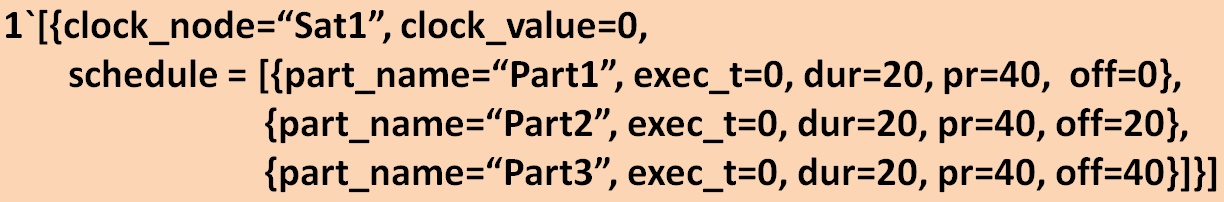
\includegraphics[width=\textwidth]{./img/clock}
	\caption{A Clock Token with Temporal Partitioning}
	\label{fig:clock}
\end{figure}

These extended data structure fields can be more easily manipulated and used by the model transitions during state changes, allowing for richer modeling concepts that would not be easily attainable using token representations provided by Timed Petri Nets. The ability to pack colored tokens with rich data structures also reduces the total number of colors required by the complete model. This quantitative measure directly influences the reduced size of the resultant state space. The downside of this approach to modeling is that we have to choose a time quantum. But in practical systems this is usually not a problem, as the low-level scheduling decisions are taken by an OS scheduler based on a time scale with a finite resolution. 

Secondly, modeling time as a token allows for smarter time progression schemes that can be applied to control the pace of simulation. If we did not have such control over time, the number of states recorded for this color token would eventually explode and itself contribute to a large state space. In order to manage this complexity, we have devised some appropriate \emph{time jumps} in specific simulation scenarios. 

If the rate at which time progresses does not change, then for a 1 msec time resolution, \emph{S} seconds of activity will generate a state space of size: $SS_{size} = \sum\limits_{i=1}^{S*1000} TF_{t_i}$ where $TF_{t_i}$ is the number of state-changing CPN transition firings between $t_i$ and $t_{i+1}$. This large state space includes intervals of time where there is no thread activity to analyze either due to lack of operation requests, lack of ready threads for scheduling, or due to temporal partitioning. During such idle periods, it is prudent to allow the analysis engine to \emph{fast-forward} time either to (1) the next node-specific clock tick, (2) the next global timer expiry event, or (3) the next activation of the node-specific temporal partition (whichever is earliest and most relevant). This ensures that the generated state space tree is devoid of nodes where there is no thread activity.

\begin{figure}[h]
	\centering
	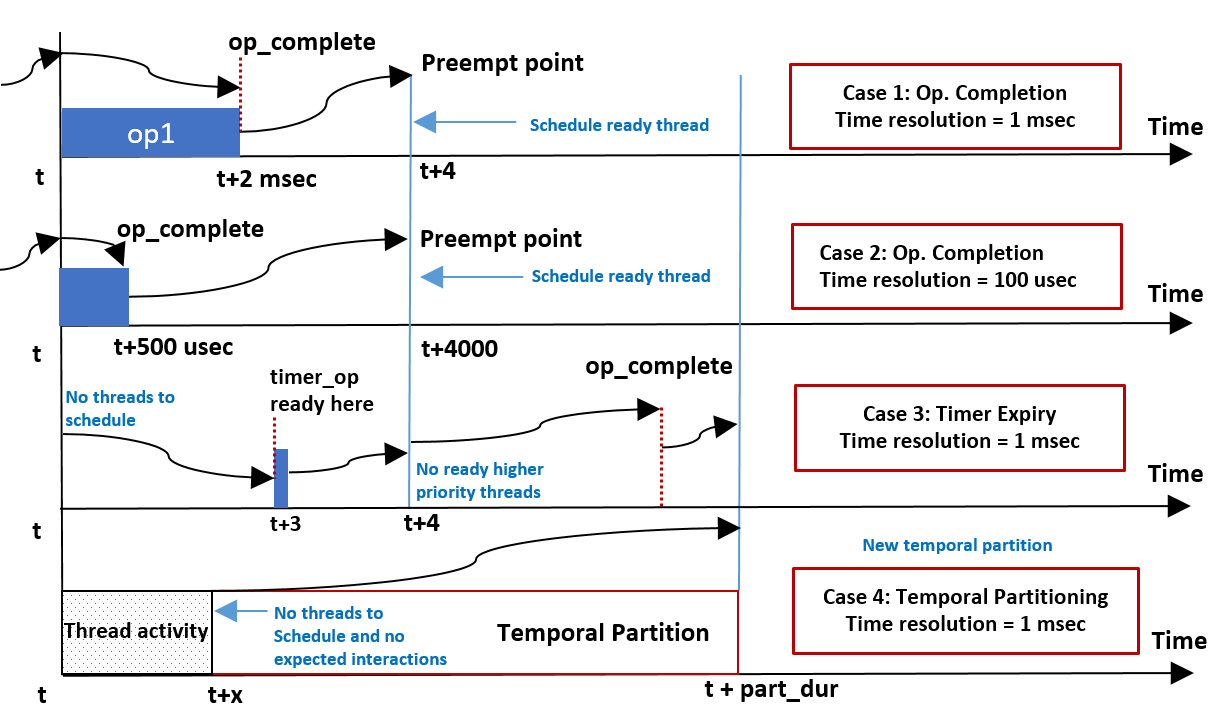
\includegraphics[width=\textwidth]{./img/time}
	\caption{Dynamic Time Progression}
	\label{fig:time}
\end{figure}

Figure \ref{fig:time} illustrates these time jumps using 4 scenarios. Assuming the scheduler clock ticks every 4 msec, Case 1 shows how time progression is handled when an operation completes 2 msec into its thread execution. At time t, the model identifies the duration of time left for an operation to complete. If this duration is earlier than the next preemption point, then there is no need to progress time in 1 msec increments as no thread can preempt this currently running thread till time t + 4 msec. Therefore, the \emph{clock\_value} in Figure \ref{fig:clock} progresses to time t + 2 msec, where the model handles the implications of the completed operation. This includes possibly new interactions and operation requests triggered in other components. Then, time is forced to progress to the next preemption point where a new candidate thread is scheduled. This same scenario is illustrated in Case 2 when the time resolution is increased to 100 usec instead of 1 msec. Notice that the number of steps taken to reach the preemption point are the same, showing how the state space doesn't have to explode simply because the time resolution is increased. Case 3 illustrates the scenario where at time t, the scheduler has no ready threads to schedule since there are no pending operation requests but at time t + 3 msec, a component timer expires, triggering an operation into execution. Since timers are maintained in a global list, each time the \emph{Progress\_Time} transition checks its firing conditions, it checks all possible timers that can expiry before the next preemption point. So, at time t when no threads are scheduled, the model immediately jumps to time t + 3. This scenario also shows that if the triggered operation does not complete before the preemption point \emph{and} there are no other ready threads or timer expiries that can be scheduled, the clock value jumps to the operation completion. It must be noted here that this case is valid only because the DREMS architecture we have considered uses a non-preemptive operation scheduling scheme. Lastly, Case 4 shows time jumps working with temporal partitioning. At some time t + x, the model realizes the absence of ready threads and does not foresee any interaction requests from other components, then it safely jumps to the end of the partition without stepping forward in 1 msec increments. This time progression directly shows how the state space of the system execution reduces while still preserving the expected execution order, justifying our choice of modeling time as a colored token using CPN. 

\subsection{Distributed Deployment} 
\label{distributed_deployment}

The second structural change to the analysis model is in how distributed deployments are modeled and simulated. Early designs on modeling and analysis of distributed application deployments \cite{kumar2014colored} included a unique token per CPN place for each hardware node in the scenario. Since the individual \emph{node} tokens are independent and unordered, there is nondeterminism in the transition bindings when choosing a hardware node to schedule threads in. For instance, if there are 2 hardware nodes in the deployment with ready threads on both nodes, then either node can be chosen first for scheduling threads leading to two possible variations of the model execution trace. Therefore the generated state space would exponentially grow for each new hardware node. In order to reduce this state space and improve the search efficiency, we have merged hardware node tokens into a single \emph{list} of tokens instead of a unassociated grouping of individual node tokens. This approach is inspired by the symmetry method for state space reduction \cite{Kristensen2000}.

\begin{figure}[h]
	\centering
	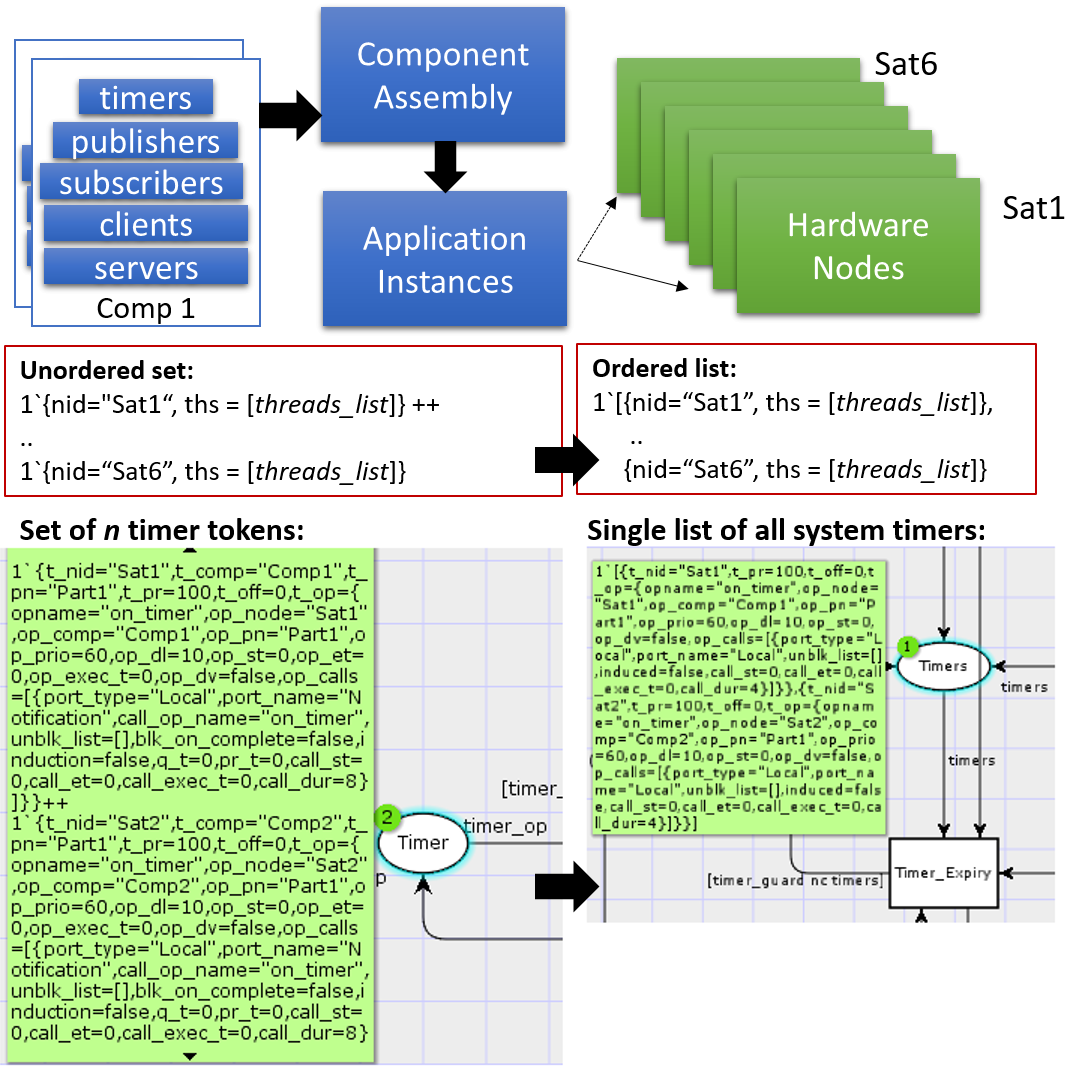
\includegraphics[width=0.8\textwidth]{./img/dd}
	\caption{Structural Reductions in CPN}
	\label{fig:dd}
\end{figure}

Figure \ref{fig:dd} illustrates this structural reduction. Consider a distributed deployment scenario with an instance of a DREMS application deployed on each hardware node, Sat1 through Sat6. Components \emph{Comp1} and \emph{Comp2} are triggered by timers, eventually leading to the execution of component operations (modeled as shown in Figure \ref{fig:ebnf}). If all the timer tokens in the system were modeled individually, the transition \emph{Timer\_Expiry} would non-deterministically choose one of the two timer tokens that are ready to expire at \emph{t=0}. However, if the timers are maintained as a single list, then this transition (1) consumes the entire list, (2) identifies all timers that are ready to expire, (3) evaluates the timer expiration function on all ready timers, (4) propagates the output \emph{operation} tokens to the relevant component message queues in a single firing. This greatly reduces the tree of possible transition firings and therefore the resultant state space. Also, if there is no non-determinism in the entire system, i.e., there is a distinct ordering of thread execution, then this model can be scaled up with instantiating the application on new hardware nodes with no increase in state space size. This is because all of the relevant tokens on all nodes are maintained as a single list that is completely handled by a single transition firing. 

An important implication of the above structural reduction is that the simulation of the entire system now progresses in synchronous steps. This means that at time 0, all the timers in all hardware nodes that are ready to expire will expire in a single step. Following this, all operations in all component message queues of all these nodes are evaluated together and appropriate component executor threads are scheduled together. When these threads execute, time progresses as described in Section \ref{handling_time}, moving forward by the minimum amount of time that can be fast-forwarded.

\newpage
\section{Investigating Advanced State Space Analysis Methods}

\subsection{Problem Statement}
State space analysis techniques have been successfully applied with Colored Petri Nets in a variety of practical scenarios and industrial use cases \cite{CPN_0}, \cite{CPN_1}. The basic idea here is to compute all reachable states of the modeled concurrent system and derive a directed graph called the state space. The graph represents the tree of possible executions that the system can take from an initial state. It is possible from this directed graph to verify behavioral properties such as queue overflows, deadline violations, system-wide deadlocks and even derive counterexamples when arriving at undesired states. 

Advanced state space analysis techniques arise from the need for efficient space space searching algorithms. State space analysis is challenged by time, memory, and computational power. Large state spaces require large CPU RAM and efficient search methodologies to quickly arrive at a useful result. With increasingly complexity in system designs, the number of state variables to store in memory also increases. Our problem here is to identify and apply advanced state space analysis techniques, applicable in the context of our CPN model and available as tested analysis tools that mitigate such complexities in state space analysis. This will help improve the scalability of our model and also reduce the memory footprint of the analysis. 

\subsection{Outline of Solution}

The variety of CPN-specific state space reduction techniques \cite{CPN_Sweepline}, \cite{CPN_Symmetry} developed in recent times has significantly broadened the class of systems that can be verified. In order to easily apply such techniques to our analysis model, we use the ASAP \cite{ASAP} analysis tool. The tool provides for several search algorithms and state space reduction techniques such as the \emph{sweep-line method} \cite{Christensen2001} which deletes already visited state space nodes from memory, forcing on-the-fly verification of temporal properties. The main advantage of such techniques is the amount of memory required by the analysis to verify useful properties for large models. 

The sweep line method for state space reduction is used to check for important safety properties such as lack of deadlocks, timing violations etc. using user-defined model-specific queries. Practical results enumerated in \cite{Christensen2001} show improvements in time and memory requirements for generating and verifying bounded state spaces. The method relies of discarding generated states on-the-fly by performing verification checks during state space generation time. Any state that does not violate system properties can be safely deleted. Another advantage of this method compared to similar reduction methods such as bit-state hashing \cite{CPN_Bitstate_Hashing} is that a complete state space search is guaranteed. 

\subsection{Evaluation of Solution}
We have evaluated these advanced state space analysis methods by comparing the obtained results with our basic state space analysis in CPN Tools. Using several criteria such as state space generation time, state space query generation, query processing time, memory usage etc., we can generate a comparison table to show the overall improvements in the analysis workflow. Advanced analysis techniques are usually accompanied by some expertise requirements that can be masked by nicely designed analysis tools. Our goal with ASAP is to use a model-driven approach to enable advanced analysis methods that does not require much expertise. With ASAP, we are able to generate verification project templates i.e. building blocks much like Simulink that are wired up together and provide an interface to the low-level analysis engine. Therefore, evaluation of this work requires both the evaluation of the advanced methods applied, and the tool used. As for the analysis methods applied, it is important to ensure that the state space tree, with all of the applied analysis heuristics, is still sufficiently probed when searching for system properties. Heuristics that enable state space analysis but only by partially checking the tree can lead the case where the state space analysis does not identify timing errors because of the incomplete search. This will be checked with negative test cases where the design model is known to be flawed; if the results from ASAP identify injected timing errors for all test cases, then the analysis is sound. 

\subsection{Contributions}
These methods were evaluated on our CPN analysis method and the results were presented in \cite{SEUS}. We used a large and diverse 100 component-based application for our testing. Using the CPN Tools' built-in state space analysis tool, a bounded state space of thread activity was generated. The state space generation took 36 minutes on a typical x86 laptop. We imported the same CPN analysis model onto ASAP and performed on-the-fly verification checks for lack of dead states in the analysis model for the same bounded state space. The on-the-fly verification, without any graphical interface overheads, took less than 10 minutes to compute a lack of system-wide deadlocks. It must be noted here that this improved result is due to not only because of the efficient state space search but also because of symmetry-based structural reduction discussed in the previous section.

In order to illustrate the utility of such state space reduction techniques, we consider a large-scale deployment. Figure \ref{fig:gm} shows the generated CPN model for a domain-specific DREMS application. This is a scaled-up variant of several satellite cluster examples we have used in previous publications \cite{DREMS13Software, kumar2014colored}. The example consists of a group of communicating satellites hosting DREMS applications. The component assembly for this application consists of 100 interacting components distributed across 10 computing nodes, many of which are triggered by infrastructural timers. Notice in Figure \ref{fig:gm} how there is only one token in each of the main CPN places, as described in Section \ref{distributed_deployment}. All of the component timers are appended to the list maintained in \emph{Timers} place. Similarly, all node-specific clock tokens are maintained in place \emph{Clocks}.  

\begin{figure}[h]
	\centering
	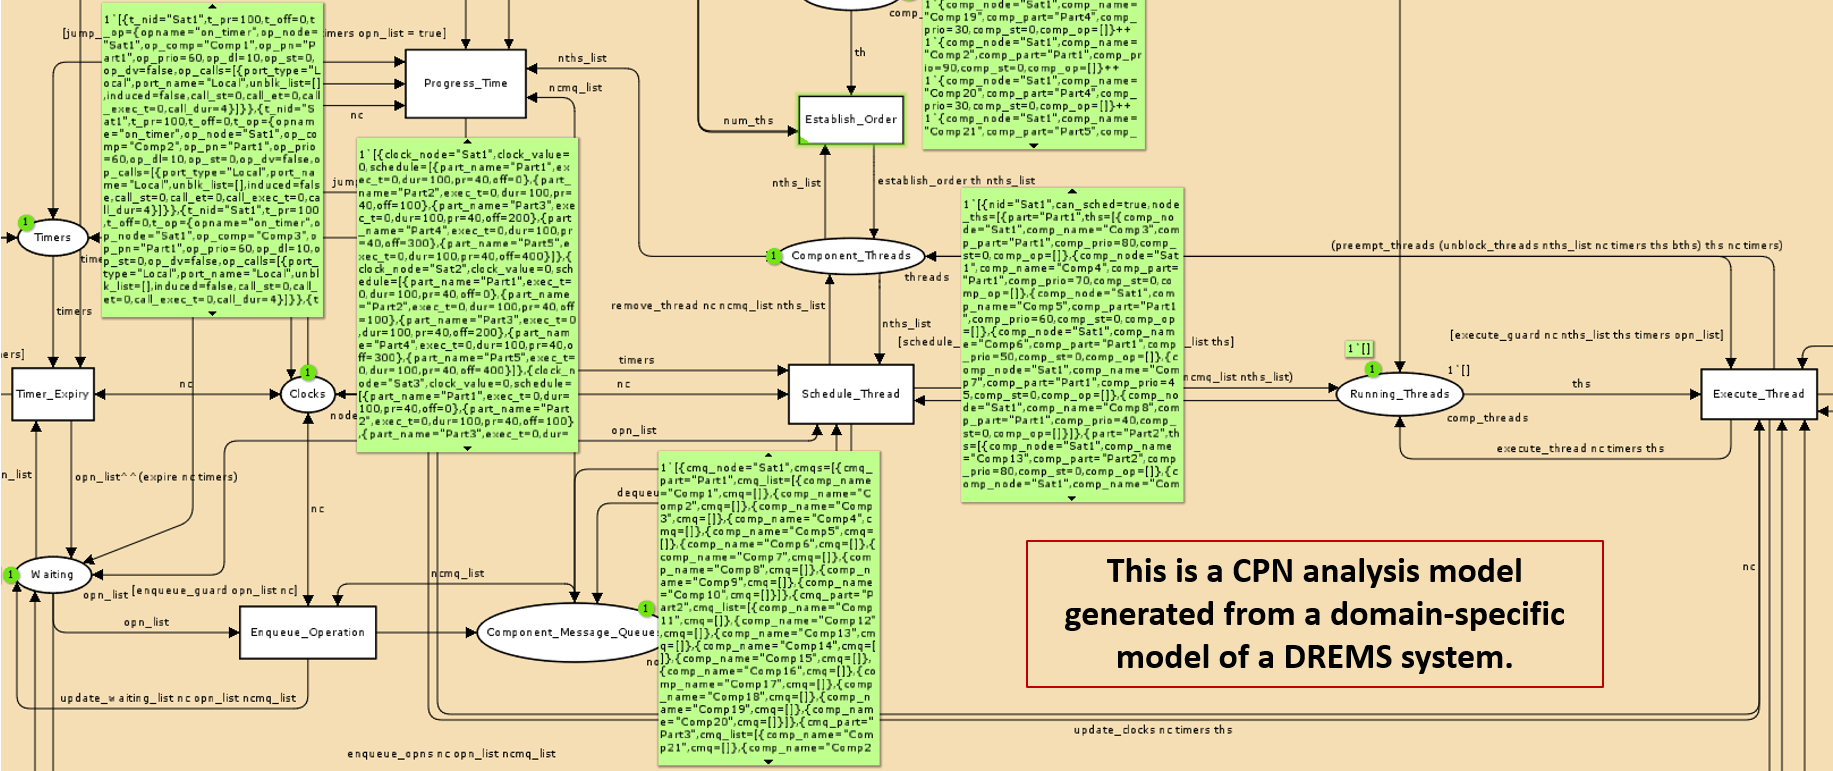
\includegraphics[width=\textwidth]{./img/Generated_Model}
	\caption{Generated CPN model for a Distributed Application Deployment}
	\label{fig:gm}
\end{figure}

At time \emph{t=0}, before the simulation is kicked off, the transition \emph{Establish\_Order} generates the powerset of thread execution orders that are possible given the configuration of the clock token. This may be a potentially large set depending on the number of threads of equal priority in each partition. Once this tree of possible orders is established, the complete set of timers that are ready to expire are evaluated. Each timer expiry manifests as an operation request and each callback operation modeled using the grammar shown in Figure \ref{fig:BL_Model}. Once the operations are ready to execute, the highest priority component thread with a pending operation request is chosen for execution. This thread scheduling happens on all hardware nodes. When each thread executes, new interactions may occur as a consequence of the execution. For instance, if a component thread executes a timer operation in which the component publishes on a global topic, the consequence of this action would include a set of callback operation requests on all components that contain subscribers to that global topic. Lastly, all running threads are evaluated to identify the minimum amount of time that can be safely fast-forwarded in each node. If the running component threads are independent or symmetrical, then the maximum possible time progression is up to the end of the temporal partition. Note here that temporal partition in the deployment can be set to an empty list which simply removes the  partitioning constraint and treats all component threads on a node as candidate threads for execution. The above sequence of transitions repeat for as long as there is a timer expiry, a pending operation request or an unfinished component interaction. 

\begin{figure}[h]
	\centering
	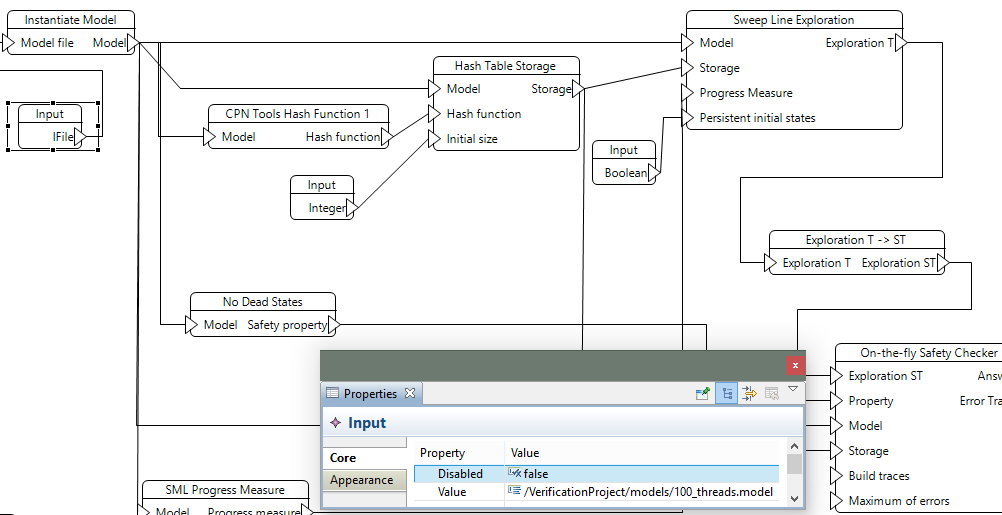
\includegraphics[width=\textwidth]{./img/sl}
	\caption{Sweep-Line Method}
	\label{fig:sl}
\end{figure}

Using the CPN Tools' built-in state space analysis tool, a bounded state space was generated reaching up-to 20 hyperperiods of component thread activity. This bounded generation took 36 minutes on a typical laptop. Our goal with such an example is to evaluate the effectiveness and utility of state space reduction techniques with respect to speed and memory usage. Figure \ref{fig:sl} shows a simple block diagram of the sweep-line method as configured in ASAP. Performing on-the-fly verification checks for lack of dead states in the analysis model, results indicate lack of system-wide deadlocks due to blocking behaviors triggered by RMI-style synchronous peer-to-peer interaction patterns. Figure \ref{fig:ds} shows analysis results obtained from a \emph{Verification Job} executed in the tool. Notice the on-the-fly verification taking less than 10 minutes to perform deadlock checks on this sample deployment. Using the \emph{Palette} in ASAP, several standard ML (SML) user queries can be created to check for domain-specific properties. 

\begin{figure}[h]
	\centering
	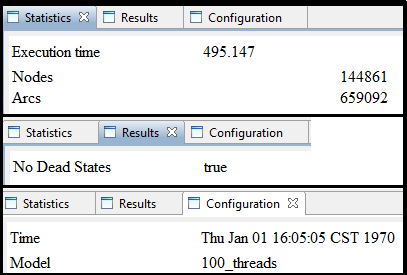
\includegraphics[width=0.6\textwidth]{./img/asap}
	\caption{Dead States Checking in a Component-based application}
	\label{fig:ds}
\end{figure}

It must be noted here that this improved result is due to not only because of the efficient state space search but also because of symmetry-based structural reduction discussed in the previous section. If not for this reduction, the state space search requirements would exponentially grow for each new hardware node added to the deployment. 
\section{Future Work}
\label{sec:Future_Work}

The DREMS component communication is facilitated by a time-varying network. The bandwidth provided by the system therefore predictably fluctuates between a minimum and a maximum during the orbital period of the satellites. Currently, our analysis associates each operational step with a fixed worst-case network delay. We are working on introducing places in the CPN model that capture the \emph{network profile} of a deployment so that the communication delays during queries vary with time leading to tighter bounds on predicted response times.   

Secondly, we are also investigating the utility of this approach for fault-tolerant and self-adaptive systems. Integrating this analysis with a run-time resilience engine, configuration changes determined by a fault mitigating solver can be subsequently checked for timing anomalies before settling on a specific reconfiguration strategy. 
\section{Conclusions}
\label{sec:Conclusions}

Mobile, distributed real-time systems operating in dynamic environments, and running mission-critical applications must satisfy strict timing requirements to operate safely. To reduce the development and integration complexity for such systems, component-based design models are being increasingly used. Appropriate analysis models are required to study the structural and behavioral complexity in such designs. 

This paper presents a Colored Petri net-based approach to capture the architecture and temporal behavior of such component-based applications for both qualitative and quantitative schedulability analysis. The analysis method is modular, extensible and intuitive and there are sufficient support tools to enable state space analysis and verification for medium to large size design models. We have  investigated the challenges faced in preemptive and non-preemptive hierarchical scheduling schemes and the effect of component interaction patterns on real-time thread execution. 


%This analysis model includes a compact, scalable representation of high-level design, accounting for the dynamics of real-time thread execution while exploiting knowledge of component execution code. Exhaustive state space search enables verification and validation of useful and necessary system properties, reducing development costs and increasing reliability for such time-critical systems. The utility of this tool has been illustrated with several examples.

\textbf{Acknowledgments:} The DARPA System F6 Program and the National
Science Foundation (CNS-1035655) supported
this work. Any opinions, findings, and conclusions or recommendations expressed
in this material are those of the authors and do not reflect the views of
DARPA or NSF. 
% \vspace{-0.1in}
\balance
\begin{spacing}{0.88}
\bibliographystyle{IEEEtran}
\bibliography{../bibliography/f6}
\end{spacing}

\end{document}
